\chapter{Scientific Background}\label{2}
An outline of the scientific concepts required for this thesis work is presented in this chapter. Firstly, the basics of wind energy conversion systems are explained. All components that are a part of an offshore wind farm network are depicted and explained. The conventional control topologies in the \gls{PE} converters of \gls{WG}s are also explained.

\section{Wind Energy Conversion Systems (WECS)}\label{WECS_theory}
The \gls{WECS} is a mixture of various engineering fields such as mechanical, electrical and control systems. The \gls{WECS} consists of several components that convert the kinetic energy of the wind into electrical energy and transfer power efficiently and systematically. The major mechanical equipment in the \gls{WECS} are the turbine tower, nacelle, rotor blades, hub, drives, gearbox, drive-train and mechanical brakes \cite{manwell2010wind}. The \gls{PE} converters, electrical generator, transmission cables, power transformers and transmission towers constitute the electrical part. The control systems govern both the electrical and mechanical systems \cite{yaramasu_high-power_2015}.
The basic structure of the \gls{WECS} is depicted in Figure \ref{fig:WECS}.   

\begin{figure}[H]
\centering
%\hspace*{-1.2cm}
    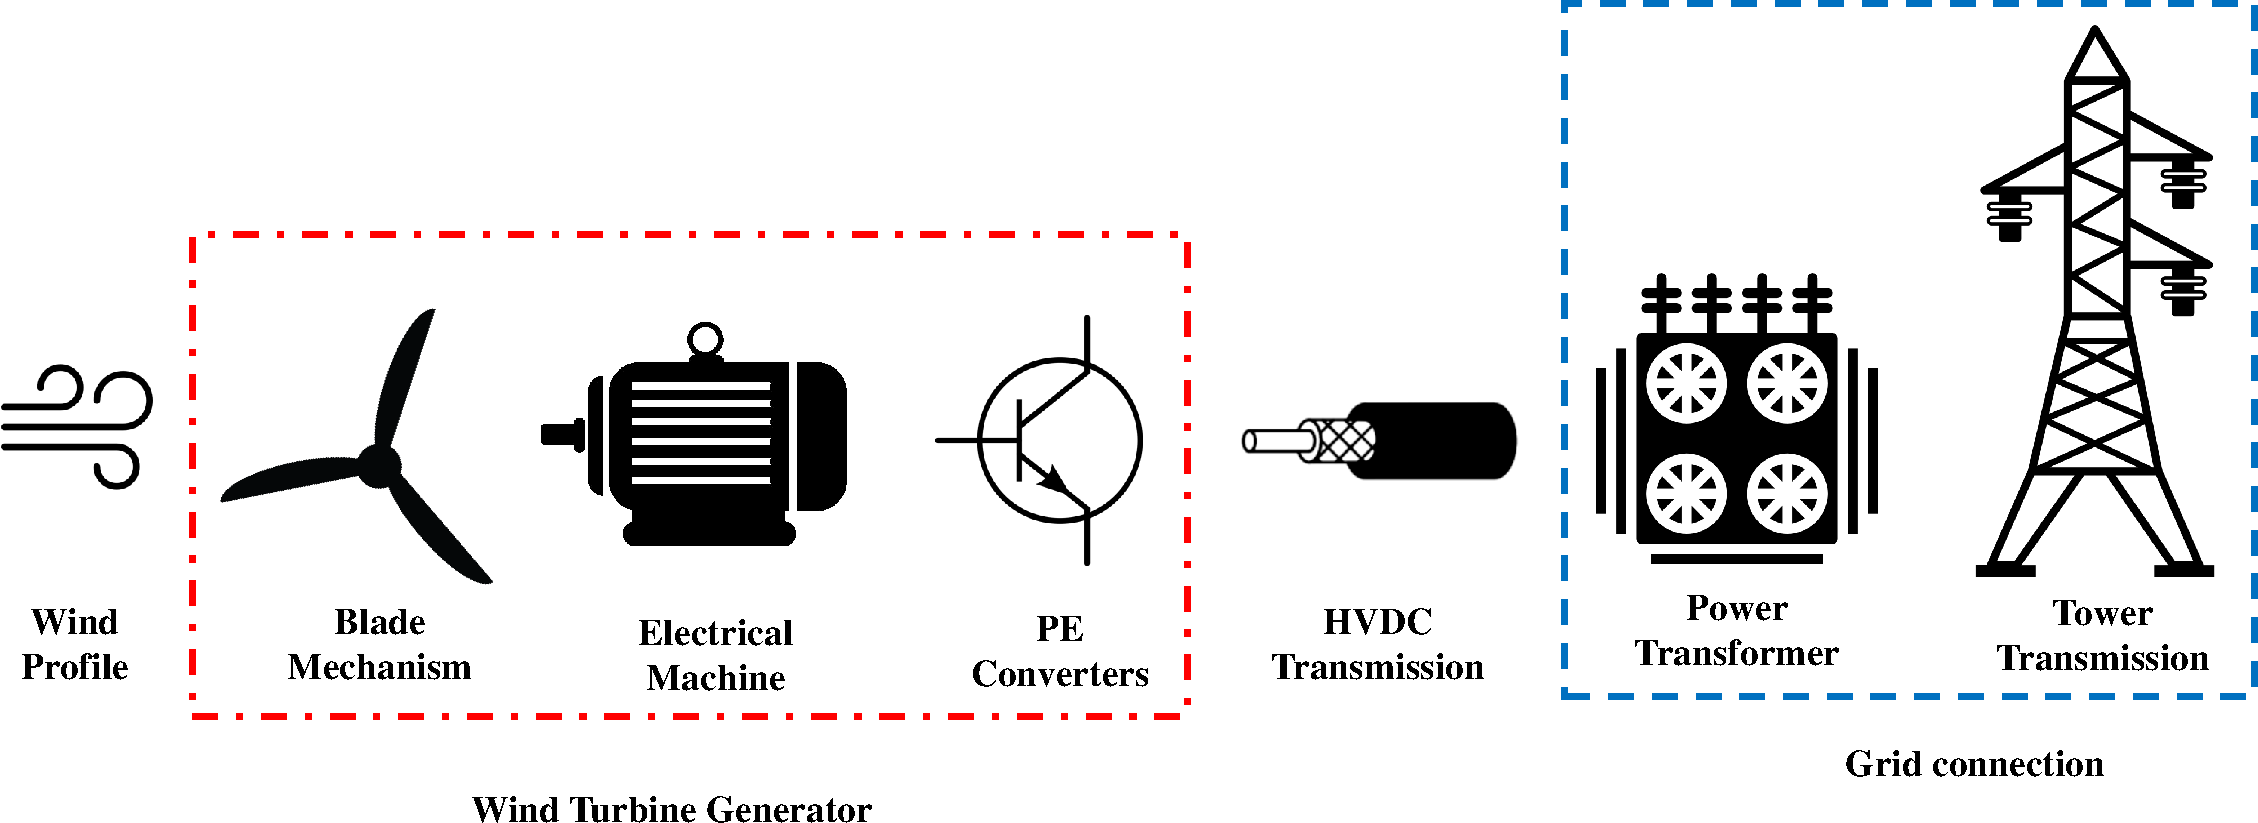
\includegraphics[height = 6.5cm,width = \textwidth]{Diagrams/Chapter_2/WECS.pdf}
    \caption{Schematic of offshore wind power transmission}
    \label{fig:WECS}
\end{figure}

\section{Power from Wind Energy} 
The wind energy converts kinetic energy of the wind to mechanical energy or electrical energy. Wind energy is represented as the kinetic energy of moving air mass. The mechanical power extracted from practical wind turbines can be depicted as in Equation \ref{windenergy} \cite{ali_wind_2012}.

\begin{equation}\label{windenergy}
    P_m =\frac{1}{2} C_p(\lambda,\beta) \rho A v_m^3 = C_p P_w
\end{equation}

where $P_m$ is the power from wind, $C_p$ is the power coefficient, $\lambda$ is the tip speed ratio, $\beta$ is the blade pitch angle in degrees, $\rho$ is the air density and $v_m$ being wind speed. 

The tip speed ratio, $\lambda$ is defined as,
\begin{equation}
\lambda= \frac{R\omega}{v} 
\end{equation}
where R is the turbine blade radius in meters and $\omega$ is the mechanical angular velocity in rad/s and $v$ is the wind speed in m/s.    

The coefficient of performance, $C_p$, is not a constant value and is a function of $\lambda$ and $\beta$. The $C_p$-$\lambda$ characteristics are represented for different pitch angle ($\beta$) values in Figure \ref{fig:pitchangle}. As can be seen, there exists a maximum mechanical power that can be achieved for a specific tip speed ratio and pitch angle.

\begin{figure}[H]
\centering
%\hspace*{-1.2cm}
    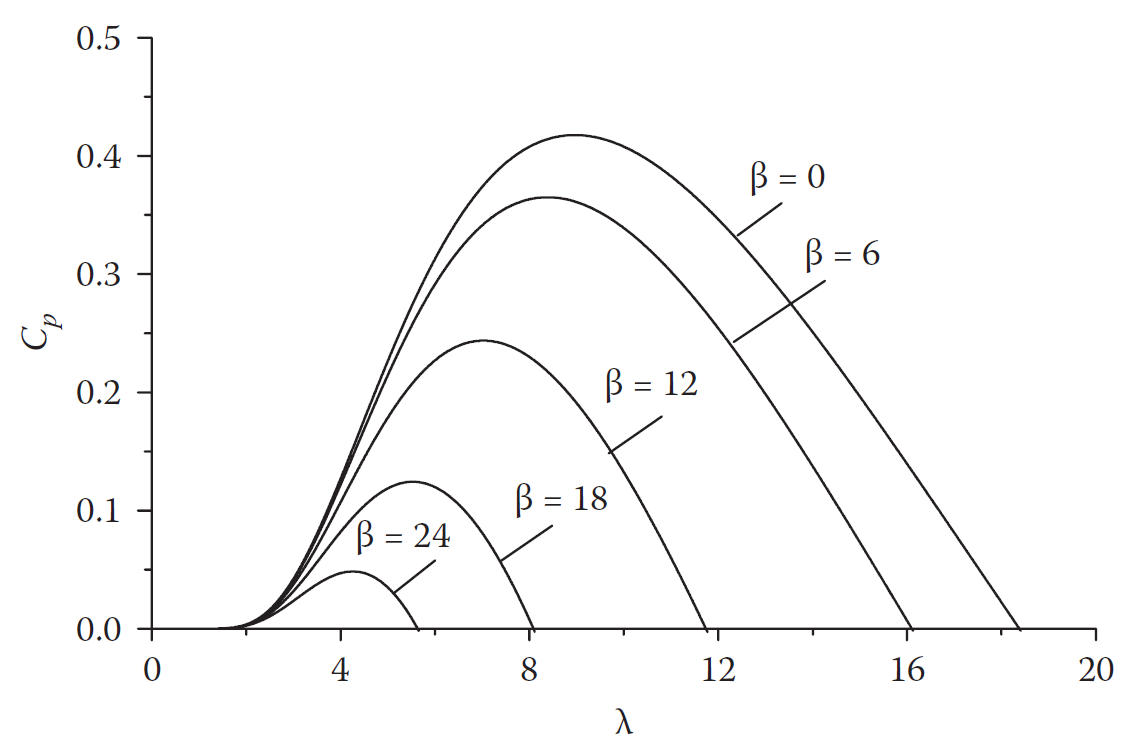
\includegraphics[height = 7.5cm,width = 11.5cm]{Diagrams/Chapter_2/pitchangle_1.png}
    \caption{Characteristics of $C_p$-$\lambda$ for various pitch angle \cite{ali_wind_2012}}
    \label{fig:pitchangle}
\end{figure}

\section{Wind Turbine Generator}
The Wind Turbine Generator (also termed as Wind Generator (\gls{WG}) ) consists of the mechanical equipment, the electrical generator and the \gls{PE} converters mentioned in Section \ref{WECS_theory} and depicted in Figure \ref{fig:WECS}. Depending on the speed of operation, \gls{WG}s can be classified as follows \cite{ali_wind_2012}:

\begin{itemize}
    \item \textbf{Type 1 - Fixed speed Induction Generator (FSIG) :} Type 1 \gls{WG} has a fixed speed of operation. Hence, maximum power extraction at all times is not possible.
    \item \textbf{Type 2 - Slip Ring Induction Generator (SRIG) :} Type 2 \gls{WG} is a variable speed technology that uses a variable resistor in the rotor windings to adjust the rotor speed. However, the variation of speed is limited in this technology, and higher heat dissipation exists due to the variable resistance.
    \item \textbf{Type 3 - Doubly-Fed Induction Generator (DFIG) :} Type 3 \gls{WG} also comes under variable speed technology. The configuration is depicted in Figure \ref{fig:Type3}. The grid transformer is directly connected to the stator of the DFIG, and the rotor is connected through a partially rated \gls{PE} converter. This configuration adds variable frequency \gls{AC} excitation (instead of only resistance) to the rotor circuit. The additional excitation for the rotor is provided through slip rings by the Voltage Source Converter (\gls{VSC}) which controls rotor currents and thereby controls the torque and reactive power of the generator. This \gls{VSC} is the Machine Side Converter (\gls{MSC}) and is connected back-to-back with a Grid Side Converter (\gls{GSC}), which provides control of the \gls{DC} link voltage and the reactive power flow to the grid. The downside of this topology is that it requires gearbox for operation and hence the chances of wear and tear is high.
    
    \begin{figure}[H]
\centering
%\hspace*{-1.2cm}
    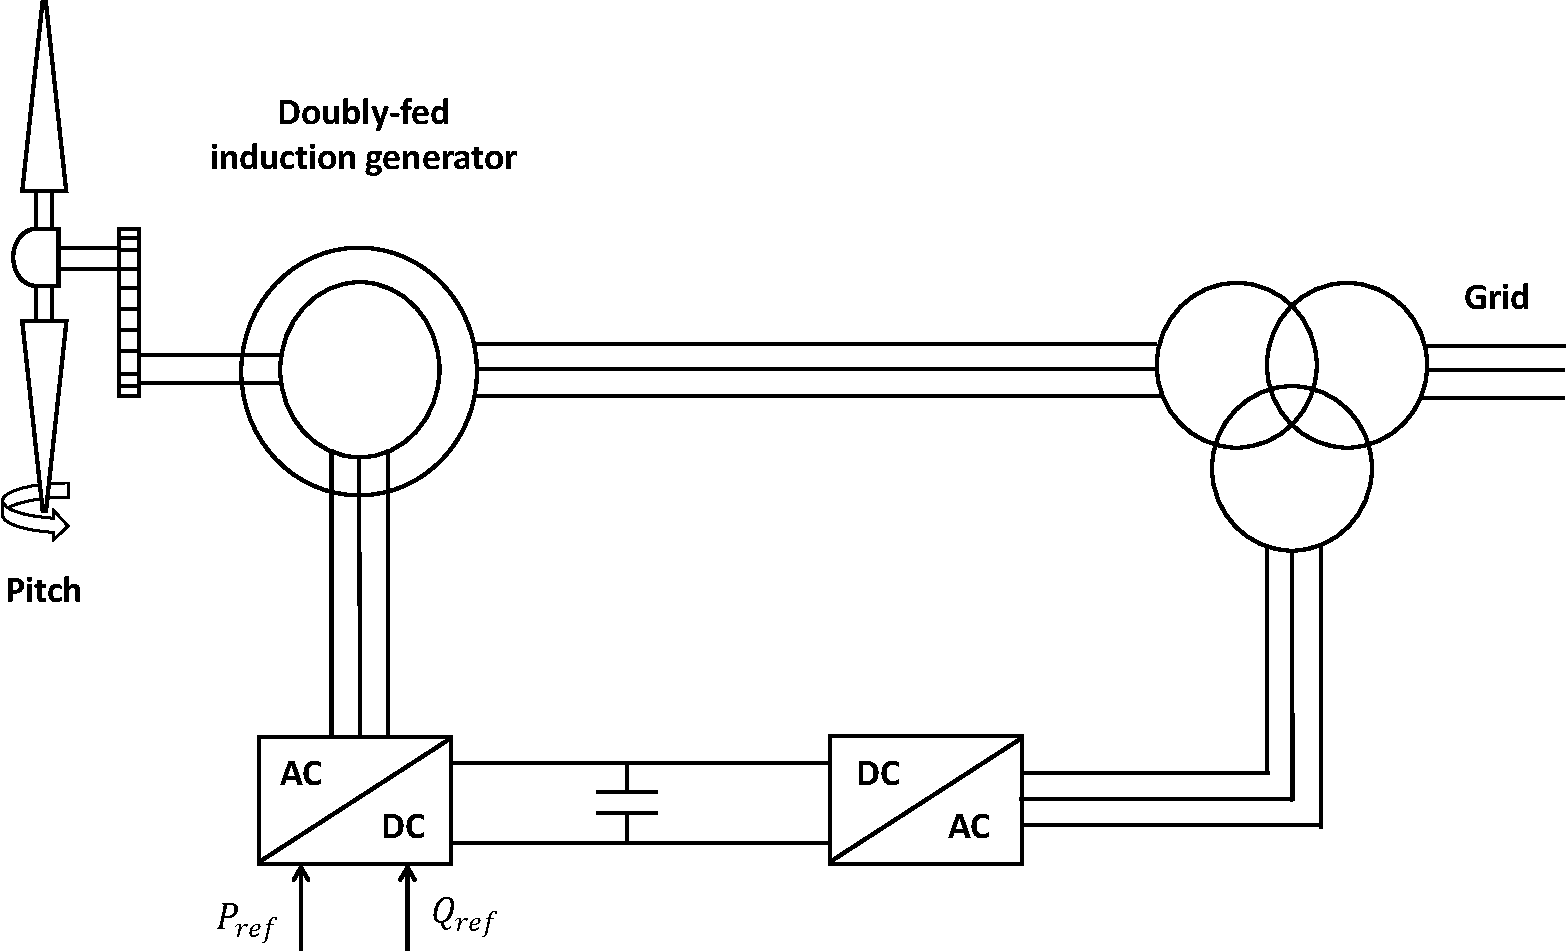
\includegraphics[height = 7cm,width = 12cm]{Diagrams/Chapter_2/Type3WT_new.pdf}
    \caption{Type 3 WG configuration \cite{ali_wind_2012}}
    \label{fig:Type3}
\end{figure}
    
    \item \textbf{Type 4 - Permanent Magnet Synchronous Generator (PMSG) :} Type-4 \gls{WG} also has a variable speed configuration, as shown in Figure \ref{fig:Type4}. \gls{PMSG} is connected to the grid transformer through a full-scale back-to-back power converter. There is no speed limit in this topology when compared to Type-3 configuration. Another advantage in Type-4 \gls{WG} is that the gearbox can be avoided. The control structures of the converters are explained in the following sections.
    
\begin{figure}[H]
\centering
%\hspace*{-1.2cm}
    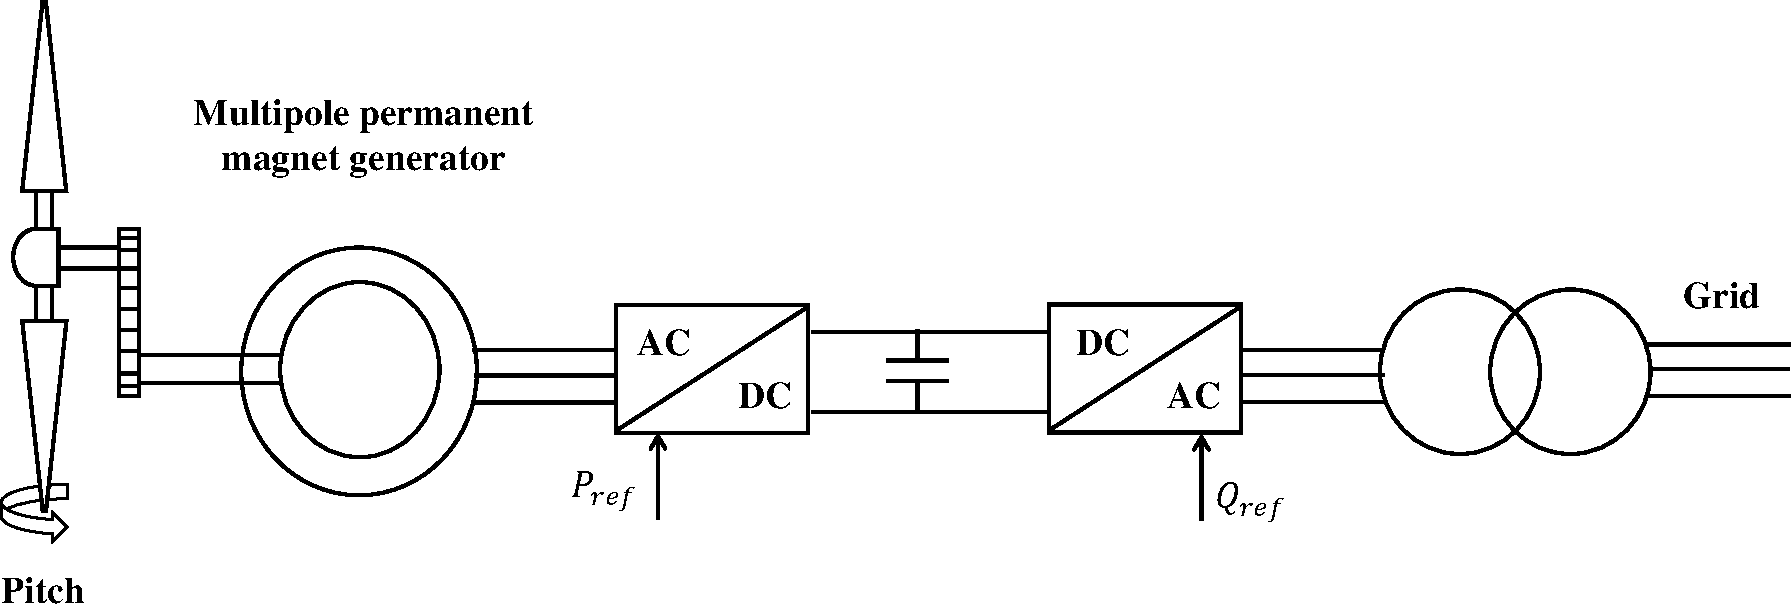
\includegraphics[height = 4.5cm,width = 13.5cm]{Diagrams/Chapter_2/Type4WT_new.pdf}
    \caption{Type-4 WG configuration \cite{ali_wind_2012}}
    \label{fig:Type4}
\end{figure}
\end{itemize}

Type-4 \gls{WG}s are employed for this thesis work, and hence the components involved for this architecture are explained further.

\subsection{Permanent Magnet Synchronous Generator (PMSG)}\label{PMSG}
As shown in Figure \ref{fig:PMSG}, \gls{PMSG} consists of stator, rotor and windings. The rotor is generally a permanent magnet that creates the magnetic flux. The stator consists of windings that are sinusoidally distributed. Generally, wound-field synchronous generators require \gls{DC} excitation to be provided by an external source. Whereas in \gls{PMSG}, external \gls{DC} excitation is not required, as it is created using the permanent magnets present in the rotor. Based on the direction of flux lines, \gls{PMSG} can be classified as radial flux, axial flux and transverse flux. Another classification is based on the location of permanent magnets on the rotor as inset \gls{PMSG}s and surface mounted \gls{PMSG}s \cite{sebastian_transient_1989}.  

\begin{figure}[]
\centering
%\hspace*{-1.2cm}
    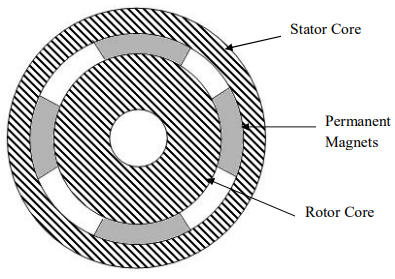
\includegraphics[height = 4.8cm,width = 7.2cm]{Diagrams/Chapter_2/PMSG.PNG}
    \caption{Cross section of a PMSG \cite{sebastian_transient_1989}}
    \label{fig:PMSG}
\end{figure}

The mathematical model of \gls{PMSG} is based on Direct-Quadrature (\gls{dq}) theory. The differential equations for the \gls{PMSG} in \gls{dq} frame are depicted in Equation \ref{PMSG_Timeeq} \cite{sebastian_transient_1989}.  

\begin{equation}\label{PMSG_Timeeq}
\begin{aligned}
    v_d = r_s . i_d + \frac{d}{dt} \Psi_d +\omega_r . \Psi_q \\
    v_q = r_s . i_q + \frac{d}{dt} \Psi_q +\omega_r . \Psi_d
\end{aligned}
\end{equation}

where $i_d$ and $i_q$ are the stator d and q axes currents respectively, $v_d$ and $v_q$ are the stator d and q axes voltages respectively. $r_s$ is the stator resistance and $\omega_r$ is electrical speed in rad/s. $\Psi_d$ and $\Psi_q$ are the d and q axes flux linkages respectively.

The flux linkages $\Psi_d$ and $\Psi_q$ are given by the Equation \ref{PMSG_psieq} \cite{rtds_tech}.

\begin{equation}\label{PMSG_psieq}
\begin{aligned}
    \Psi_d = L_d . i_d + L_{md} . i_D  + \Psi_m \\
    \Psi_q = L_q . i_q + L_{mq} . i_Q
\end{aligned}
\end{equation}

where $L_d$ and $L_q$ are the inductances in d and q axes respectively, $L_{md}$ and $L_{mq}$ are mutual inductances and $\Psi_m$ is the permanent magnet flux linkage.

%The equivalent circuit in \gls{dq} frame is shown in Figure \ref{fig:PMSG_equiv_ckt}. 

% The effects of permanent magnets are represented by a current source in the d-axis circuit. Equation \ref{Currentsource_MagFluxeq} shows the correspondence between the current source and the permanent magnet flux linkage.

% \begin{equation}\label{Currentsource_MagFluxeq}
%     \Psi_m = L_{md} . i_m
% \end{equation}

% \begin{figure}[H]
% \centering
% %\hspace*{-1.2cm}
%     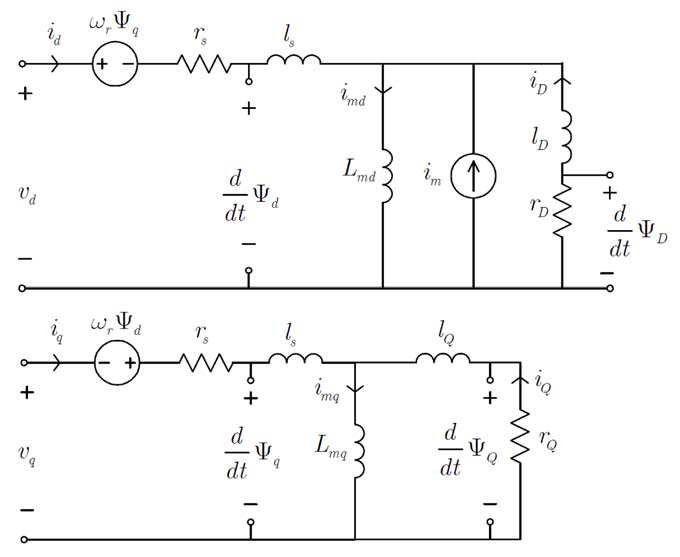
\includegraphics[height = 6.5cm,width = 8.5cm]{Diagrams/Chapter_2/PMSG_equiv_ckt.png}
%     \caption{d and q axes equivalent circuit of PMSG \cite{sebastian_transient_1989}}
%     \label{fig:PMSG_equiv_ckt}
% \end{figure}

\subsection{Voltage Source Converter (VSC)}\label{VSC_theory}
The stator of the \gls{PMSG} is connected directly to the \gls{AC} side of a \gls{VSC} as seen in Figure \ref{fig:Type4}. This \gls{VSC} which works as a rectifier during generation operation is termed as \gls{MSC}. It is interfaced back to back with another \gls{VSC} that works as an inverter during generation operation and is called \gls{GSC}.

\gls{VSC} consists of self-commutated switching devices such as the Insulated Gate Bipolar Transistors (\gls{IGBT}s) and anti-parallel diodes and hence allows the bidirectional flow of power between the \gls{AC} and \gls{DC} sides. The output voltage is obtained by switching off the \gls{IGBT}s in a synchronized manner. The \gls{VSC}s are classified as two-level or multi-level depending on the number of voltage levels they can generate \cite{noauthor_appendix_2014}. 

\subsubsection{Two-level VSC}
The two-level \gls{VSC} is the most commonly used type of converter in various applications because of the simplicity of its operation. The configuration of a two-level \gls{VSC} is depicted in Figure \ref{fig:2levelVSC}. Voltages of (1/2 $V_{dc}$, -1/2 $V_{dc}$) can be obtained using two-level \gls{VSC} as shown in the graph in Figure \ref{fig:2levelVSC}. The operation of switches $S_{1}$ and $S_{2}$ in two-level \gls{VSC} are operated complementary to prevent short circuit across the \gls{DC} link, hence protecting the \gls{PE} devices from being subjected to over-current.

\begin{figure}[H]
\centering
%\hspace*{-1.2cm}
    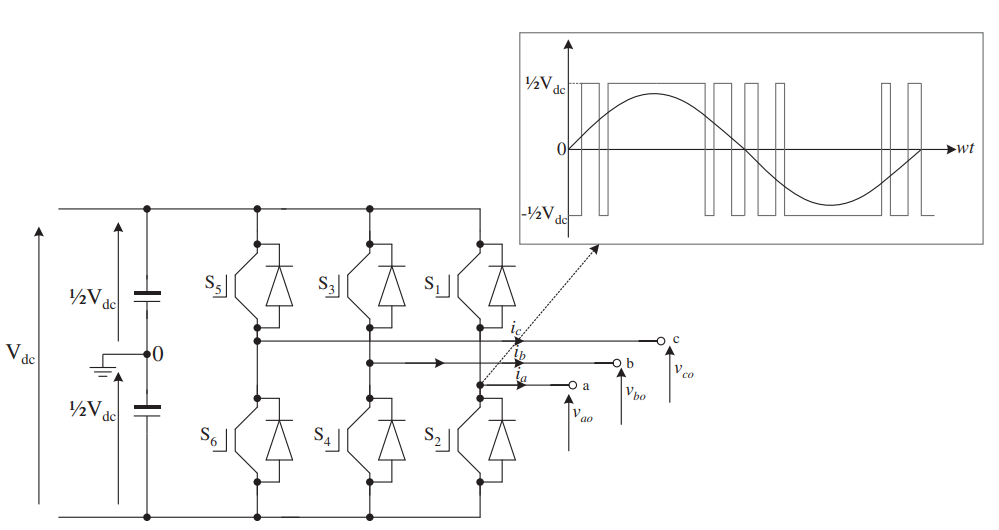
\includegraphics[height = 7.5cm,width = 15.5cm]{Diagrams/Chapter_2/2levelVSC.PNG}
    \caption{Two-level VSC \cite{noauthor_appendix_2014}}
    \label{fig:2levelVSC}
\end{figure}

\subsubsection{Multi-level VSC}
\gls{VSC}s with three or more levels are termed as multi-level \gls{VSC}s. The three-level \gls{VSC} is among the first multi-level configuration used on large scale and is also termed as Neutral Point Clamped (\gls{NPC}) converter \cite{sharifabadi2016design}. The topology of a \gls{NPC} converter is shown in Figure \ref{fig:3levelVSC}. The voltage levels of (1/2 $V_{dc}$ , 0 , -1/2 $V_{dc}$) can be obtained using a \gls{NPC} converter. This provides a better sinusoidal nature and also reduces the Total Harmonic Distortion (THD) when compared to a two-level \gls{VSC}. The switches ($S_{a1}$,$S_{a3}$) and ($S_{a2}$,$S_{a4}$) are operated complementary in a \gls{NPC} converter. This means, turning on switch $S_{a1}$ eliminates $S_{a3}$ from being turned on and the same pattern is followed for the latter complementary pair. The summary of switching operation for a \gls{NPC} converter is shown in Table. \ref{tab:3level_switching}. 

\begin{figure}[H]
\centering
%\hspace*{-1.2cm}
    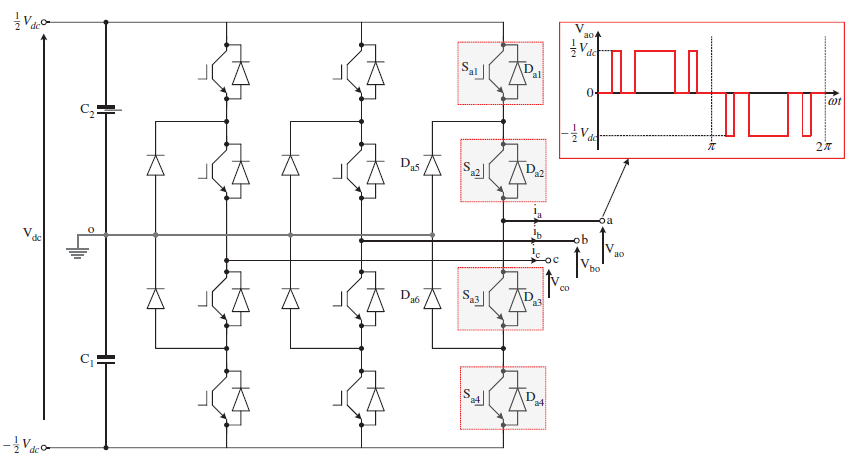
\includegraphics[height = 9cm,width = \textwidth]{Diagrams/Chapter_2/3levelVSC.PNG}
    \caption{Three-level VSC or NPC Converter \cite{noauthor_appendix_2014}}
    \label{fig:3levelVSC}
\end{figure}

\begin{table}[H]
\centering
\begin{tabular}{c|c|c|c|c|}
\cline{2-5}
                                          & \multicolumn{4}{c|}{Switch state}     \\ \hline
\multicolumn{1}{|c|}{Voltage level}       & $S_{a1}$ & $S_{a2}$ & $S_{a3}$ & $S_{a4}$ \\ \hline
\multicolumn{1}{|c|}{$\frac{1}{2}V_{dc}$}  & ON      & ON      & OFF     & OFF     \\ \hline
\multicolumn{1}{|c|}{0}                   & OFF     & ON      & ON      & OFF     \\ \hline
\multicolumn{1}{|c|}{$-\frac{1}{2}V_{dc}$} & OFF     & OFF     & ON      & ON      \\ \hline
\end{tabular}
\caption{Switching operation of a three-level VSC \cite{noauthor_appendix_2014}}
\label{tab:3level_switching}
\end{table}

\subsubsection{Pulse Width Modulation (PWM)}
The switching of the valves has to be configured using a control mechanism to ensure proper operation. To reduce the harmonic content and to control the magnitude of output voltage, many Pulse Width Modulation (\gls{PWM}) techniques are developed. Few of them used currently are, Selective Harmonic Elimination (SHE), Sinusoidal Pulse Width Modulation (SPWM) and Space Vector Modulation (SVM). SPWM technique is employed in this thesis and is explained further. SPWM is one of the simplest methods to be implemented and provides high effectiveness in modulation by suppressing the harmonic contents that are farther from the fundamental frequency component. SPWM can be termed to be a multi-pulse based modulation technique that changes the pulse width of the output voltage of the converter in a sinusoidal fashion with respect to a corresponding reference voltage. The implementation of this concept is done by comparing a particular reference signal of low-frequency with a carrier signal of higher frequency. The reference signal frequency is set to the required fundamental frequency, which is normally 50 Hz or 60 Hz, and the carrier signal frequency should be higher than the reference signal frequency. An example of SPWM in two-level \gls{VSC} is shown in Figure \ref{fig:2levelVSC_switching}.

\begin{figure}[H]
\centering
%\hspace*{-1.2cm}
    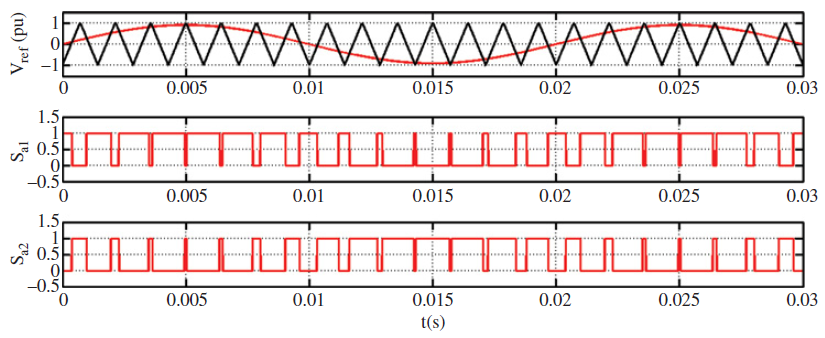
\includegraphics[height = 5.5cm,width = 13.5cm]{Diagrams/Chapter_2/2levelVSC_switching.PNG}
    \caption{SPWM for phase A in two-level VSC \cite{noauthor_appendix_2014}}
    \label{fig:2levelVSC_switching}
\end{figure}

\subsubsection{Reference frame transformation}\label{ref_frame_trafo}
\gls{PI} controllers are widely used for the control operation of \gls{VSC}s in power systems. It is therefore relevant to translate from three-phase abc frame to a rotating \gls{dq} frame in order to have a two signal representation of three-phase \gls{AC} signals. Figure \ref{fig:DQTransformation} shows the Clarke-Park transformation used for this purpose. The three-phase measured signals from the node are translated to a stationary reference frame ($\alpha \beta$) using the Clarke transform. It is then translated to a synchronous rotating \gls{dq} frame using the Park transform. The reference signal for control is provided to the corresponding frame, and after the control process is established, it is translated back to the three-phase signals. In real-world, during translation to a rotating \gls{dq} frame, the d-axis is aligned with the grid voltage, and q-axis is aligned to zero. The alignment is done by the voltage angle determined by the Phase Locked Loop (\gls{PLL}). Such an approach provides control of active power or \gls{DC} voltage using d-axis current component of the converter, while the reactive power or \gls{AC} voltage can be controlled using the q-axis current component of the converter.   

\begin{figure}[H]
\centering
%\hspace*{-1.2cm}
    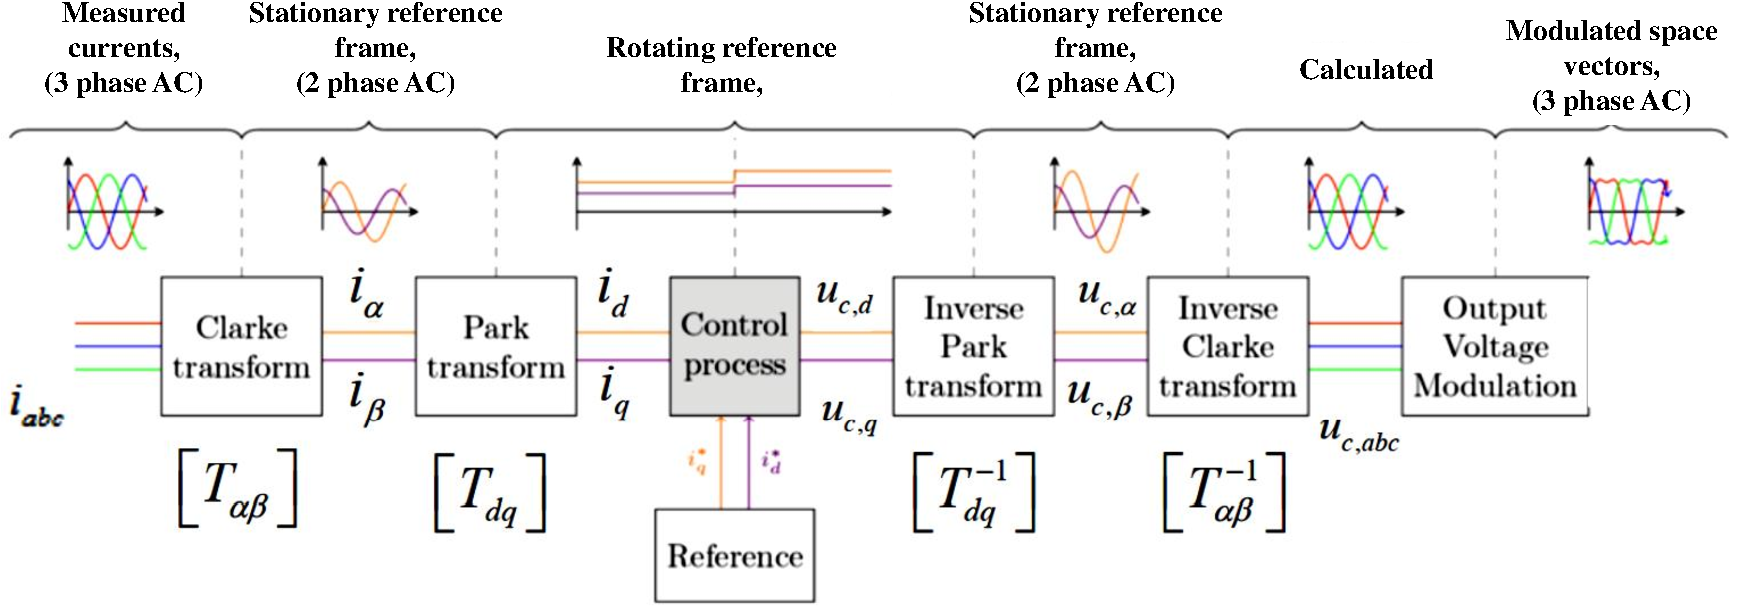
\includegraphics[height = 5.5cm,width = 15.5cm]{Diagrams/Chapter_2/DQTransformation.pdf}
    \caption{Reference frame transformation for control of VSC \cite{ndreko2017offshore}}
    \label{fig:DQTransformation}
\end{figure}

\subsection{Machine Side Converter (MSC) Control}
The \gls{MSC} controller is in charge of optimizing the rotor speed to increase the amount of wind energy being captured continuously \cite{strachan_stability_2010}. %There are several control strategies available to perform this task by achieving different objectives \cite{bose_power_2006}. 
The following equation gives the electromagnetic torque of the \gls{PMSG}.

\begin{equation}\label{elec_torque}
T_e = \frac{3}{2}P_n[\Psi_m.i_q-(L_d-L_q)i_d.i_q]    
\end{equation}

where $P_n$ is the number of pole pairs.

The majorly used mechanisms for the control of \gls{MSC} are the following three control schemes \cite{wu_variable-speed_2011}:

\begin{itemize}
    \item Zero d-axis Control (ZDC): As the name suggests, this control involves setting the d-axis component of stator current to zero. If $i_d$= 0 in Equation \ref{elec_torque}, the electromagnetic torque will be proportional to the q-axis component of stator current ($i_q$).  
    \item Maximum Torque per Ampere (MTPA) control: The concept of MTPA control is to generate a required torque with a minimum stator current. Thereby, the use of stator current is increased, and the losses across the stator windings are reduced. In case of non-salient pole generators, the inductances in d and q axes are the same ($L_d$ = $L_q$). On substituting $L_d$ = $L_q$ in Equation \ref{elec_torque}, this simplifies to the fact that electromagnetic torque is proportional to the q-axis current component. Therefore, the MTPA control is the same as the ZDC in case of non-salient pole generators. 
    \item Unity Power Factor (UPF) control: The stator voltage and current phase angles are calculated initially. To achieve UPF, the angle between the stator voltage and current, i.e. the stator power factor angle must be zero. The equations are then solved for both the d and q axes stator currents. 
\end{itemize}

Additionally, the generator is also governed by the Maximum Power Point Tracking (\gls{MPPT}) mechanism to extract the maximum power possible. There are two ways of implementing this mechanism; the first involves measuring the speed of the \gls{WG} shaft, and the maximum mechanical power that can be extracted is calculated. The error obtained by comparing the maximum mechanical power with the actual power achieved is provided for the \gls{MSC} control. The next method is through measurement of wind speed. If for a given speed, the ratio of optimum tip speed ratio and the radius of the blade is known, the optimal rotational speed of the rotor ($v\lambda_{opt}$ /R) can be calculated. The error obtained on comparing this speed with the measured speed is used to calculate the $i_{q,ref}$ component \cite{ali_wind_2012}. The detailed implementation of \gls{MSC} control in RSCAD is given in Appendix \ref{MSC_Control}.  

\subsection{Grid Side Converter (GSC) or Line Side Converter (LSC) Control}
The \gls{GSC} is connected back to back with the \gls{MSC} through a \gls{DC} link. The \gls{GSC} is mainly responsible for providing \gls{DC} voltage control and the \gls{AC} side reactive power control. 

\subsubsection{Conventional Current Control}\label{conv_current_control}
The conventional control of \gls{GSC} implemented in power systems follows the current control strategy. This involves an outer loop to control the \gls{DC} voltage ($V_{dc}$) in d-axis, and \gls{AC} voltage ($V_{ac}$) or reactive power ($Q$) control in q-axis as shown in the blue box in Figure \ref{fig:Diss_GSC_control}. The outer loop provides reference set points ($i_{d\_ref}$ and $i_{q\_ref}$) for the inner current control loop which is represented by the orange coloured box in Figure \ref{fig:Diss_GSC_control}. The inner loop consists of \gls{PI} controllers and feed-forward term ($V_T$) that form the major part of the control. The decoupling terms ($x$) are added at the end of the current regulator output to improve the dynamic performance of the system.  

The conventional current control strategy has not led to any major issues until now, because the synchronous generators in power plants were capable of absorbing the injected currents. However, this is not the case for a network that is dominantly connected using \gls{PE} interface. An example of such a situation is an \gls{OWF} network. The effect could also be severe for a large scale \gls{OWF} network involving more \gls{PE} converters to be connected to the network. Hence this calls for the need for better control strategies.

\begin{figure}[H]
\centering
%\hspace*{-1.2cm}
    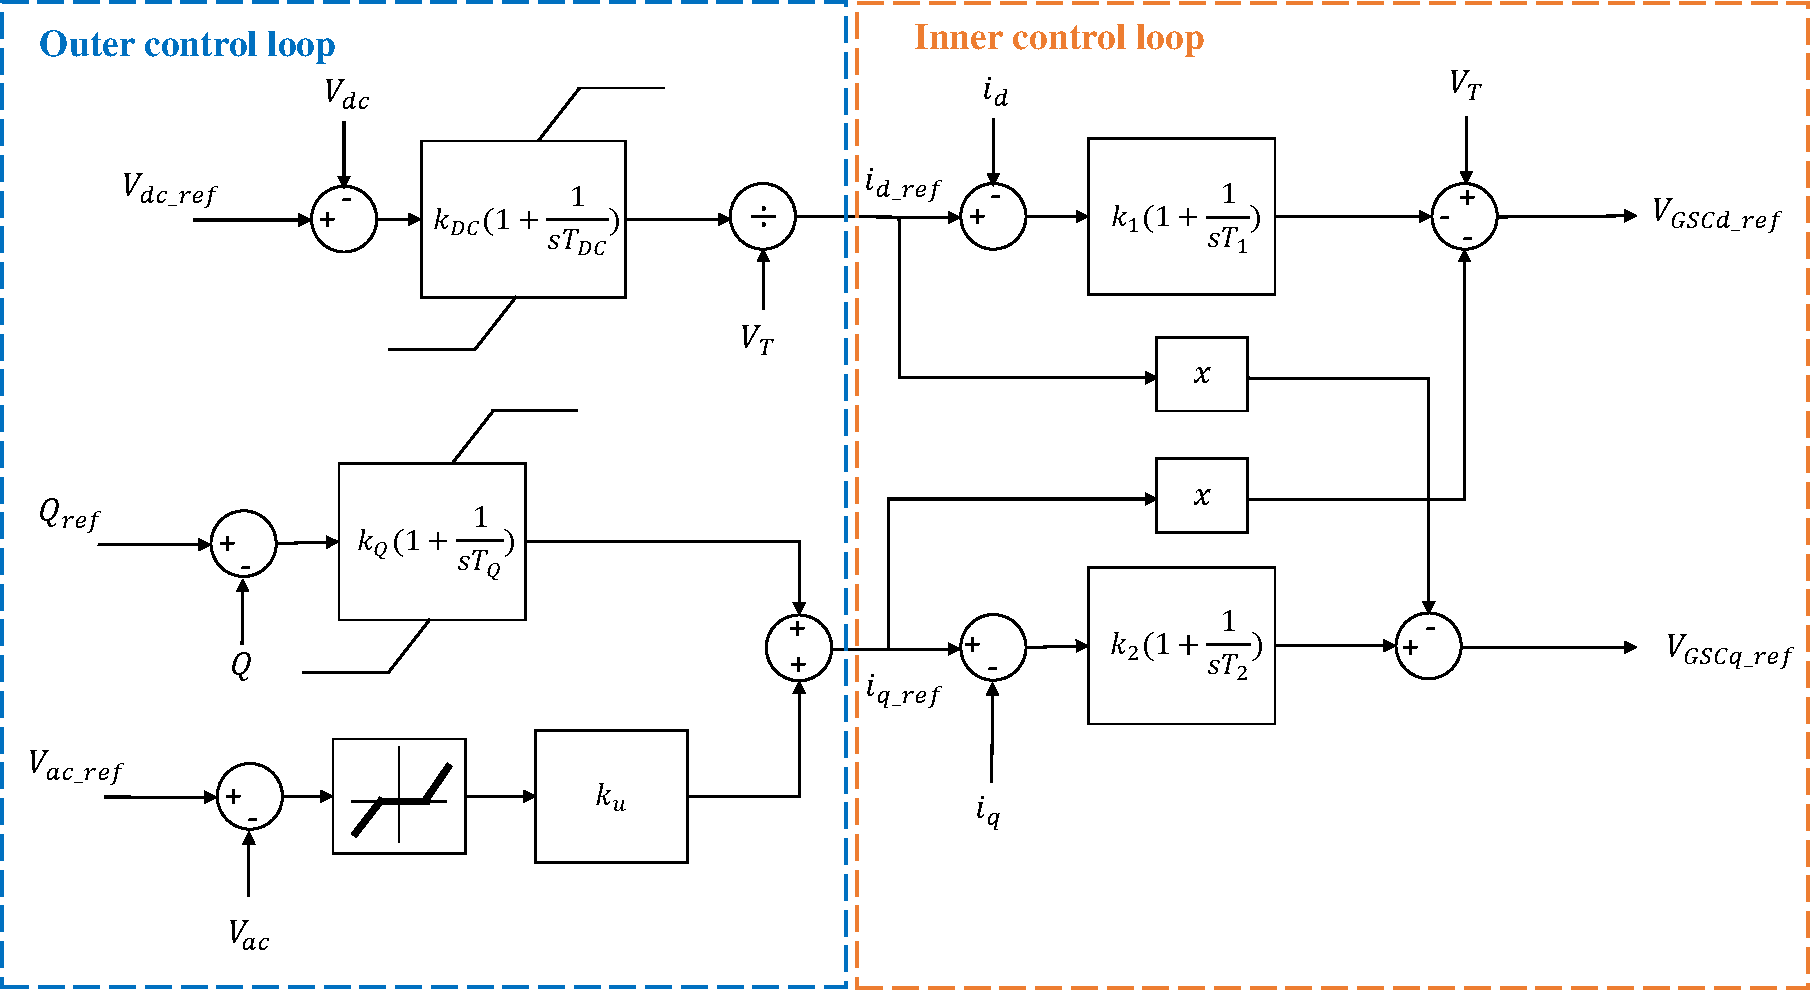
\includegraphics[height = 8.5cm,width = 15.5cm]{Diagrams/Chapter_2/Inner_control_GSC_chap2.pdf}
    \caption{Conventional current control in GSC \cite{korai_dynamic_2019}}
    \label{fig:Diss_GSC_control}
\end{figure}


\subsubsection{Direct Voltage Control (DVC)}\label{DVC_theory}
The major issue with conventional control is the wind up of the integrator that causes the voltage to rise. This happens because the reference value of current ($i_{d\_ref}$ and $i_{q\_ref}$) remains non-zero and the measured current ($i_d$ and $i_q$) following islanding nearly falls to zero. To overcome this issue, the inner control loop in Figure \ref{fig:Diss_GSC_control} is modified as shown in Figure \ref{fig:Diss_DVC_control}. In Figure \ref{fig:Diss_DVC_control}, the integrator term is avoided, and the proportional term is moved to the output end. However, this causes the set points to differ in the absence of the integral component. The main role of set points is to limit the \gls{PE} converter current. Nevertheless, the current limitation would be based on the grid situation, and hence the performance of the controller is not affected in the absence of the integral component \cite{korai_dynamic_2019}, \cite{erlich_new_2017}.       

\begin{figure}[H]
\centering
%\hspace*{-1.2cm}
    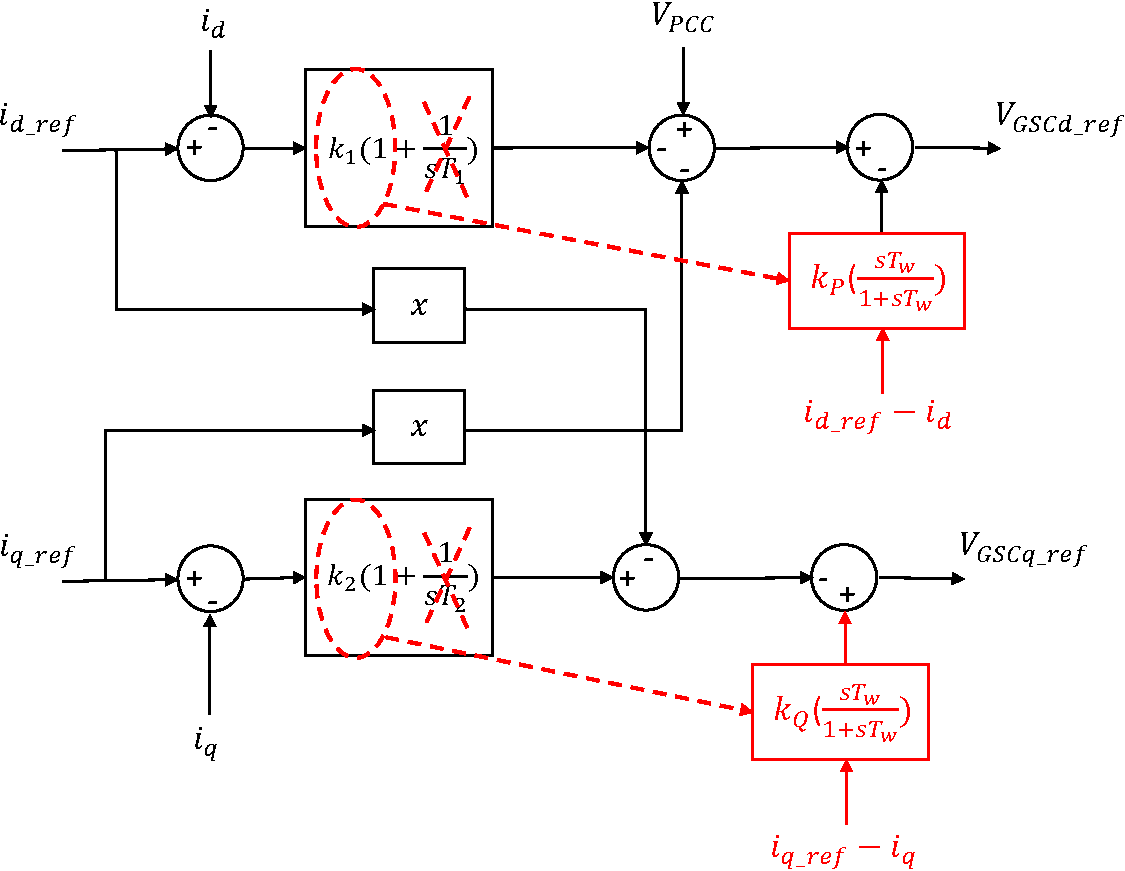
\includegraphics[height = 8.5cm,width = 10.5cm]{Diagrams/Chapter_2/Inner_control_GSC_chap2_2.pdf}
    \caption{ Development of new voltage controller strategy by modifications in the inner control loop of conventional current controller \cite{erlich_new_2017}}
    \label{fig:Diss_DVC_control}
\end{figure}

The damping of transient scenarios is provided by imitating the use of a resistor in series in the \gls{PE} converter circuit. In the real scenario, damping can be depicted as the power loss across a resistor. However, placing a physical resistor in the circuit causes loss of active power which is not desired. In order to achieve the damping effect without power loss, the controller is formulated to mimic the drop in voltage using a virtual resistor \cite{erlich_new_2017}. The value of the virtual resistors in d and q axes are the gains ($k_P$ and $k_Q$) of the washout filers depicted in red boxes in Figure \ref{fig:Diss_DVC_control}.

The control strategy developed in \cite{korai_dynamic_2019} uses a vector control strategy similar to the conventional current control. The transformation in d and q axis allows the independent control of active and reactive powers. This control strategy is adapted for this thesis and is explained in detail in Section \ref{DVC_RSCAD}. 

\subsubsection{Power balance equation}
The power balance equation at the \gls{WG} is given as follows:

\begin{equation}\label{powbaleq}
    P_{inverter,input} = P_{rectifier,output} + P_{capacitor}  
\end{equation}

where rectifier is the \gls{MSC} and inverter is the \gls{GSC}. For steady-state conditions, the voltage across the \gls{DC} capacitance is steady. Thereby, the active power input for the inverter (\gls{GSC}) equals the active power output from the rectifier (\gls{MSC}). During the fault condition, the active power output from the inverter is decreased, whereas the output from the rectifier tends to be the same. The capacitors are charged during this scenario, and the \gls{DC} link voltage increases to maintain the power balance. 

\section{High Voltage Direct Current (HVDC) Transmission}\label{HVDC_trans_theory}
As the name suggests, a High Voltage Direct Current (\gls{HVDC}) transmission system uses \gls{DC} for bulk transmission of electrical power. The electrical power from the offshore \gls{AC} network is stepped-up using a power transformer and is converted to \gls{DC} at the converter station, which is transmitted to onshore locations using subsea cables or overhead lines \cite{abbreviewnew}. The commercial utilization of \gls{HVDC} transmission was started in 1954 \cite{cigre2005b4}, \cite{peake_history_2010}. \gls{HVDC} technology employs \gls{VSC}s to convert power from \gls{AC} to \gls{DC} and vice versa, as explained in Section \ref{VSC_theory}, and hence the systems that employ this technology are termed as \gls{VSC}-\gls{HVDC} systems.

As explained in Section \ref{VSC_theory}, the classification for \gls{VSC}s can be termed as two-level and multi-level. The two-level \gls{VSC}s are an economical solution for low power rating applications up to 1 MVA. The main drawbacks of two-level \gls{VSC}s include increased power losses, high harmonic content on the \gls{AC} side voltages and require expensive filters to mitigate the harmonics. On the other hand, multi-level converters provide notable improvements for the above mentioned issues as can be seen in Figure \ref{fig:2levelVSCtoMMC} \cite{sharifabadi2016design}.   

\begin{figure}[H]
\centering
%\hspace*{-1.2cm}
    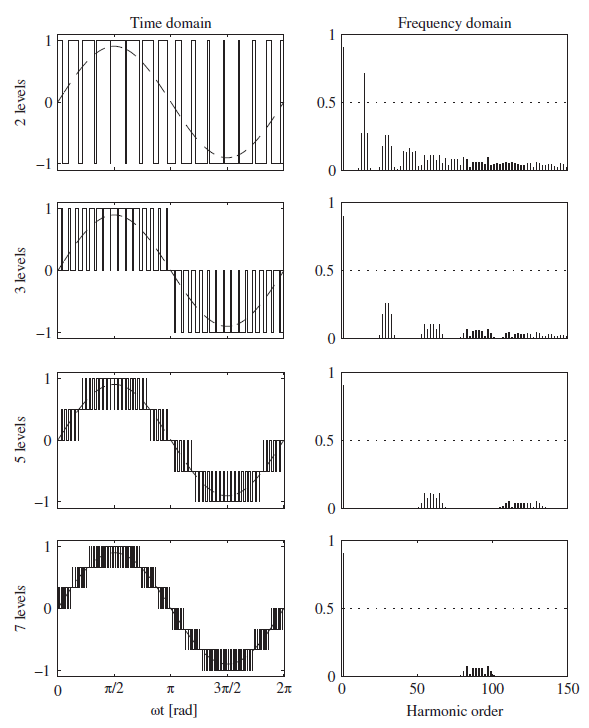
\includegraphics[height = 11.5cm,width = 10.5cm]{Diagrams/Chapter_2/2levelVSCtoMMC.PNG}
    \caption{Effect of moving towards multi-level converters \cite{sharifabadi2016design}}
    \label{fig:2levelVSCtoMMC}
\end{figure}

The most common multi-level converters for high voltage applications in recent times are the Modular Multi-level Converters (\gls{MMC})s. The significant component in an \gls{MMC} is the switching submodule that can be either half-bridge or full-bridge submodules. The half-bridge submodule has one two-level phase leg parallel to a \gls{DC} capacitor that maintains the \gls{DC} voltage. The voltage level can be increased by connecting the submodules in series. The \gls{DC} power at the output of \gls{MMC} is transmitted to the onshore converter using subsea \gls{HVDC} cables. It is converted back to \gls{AC} at the onshore converter station and sent to the distribution network.

Having understood the basics of various equipment in an \gls{OWF} and \gls{VSC}-\gls{HVDC} transmission, the goal of modelling a multi-gigawatt offshore network with identified control strategies needs to be achieved. Implementation of the control strategy for a single \gls{WG} model is taken as the starting step and is explained in the following chapter. 
